\documentclass[ngerman, aspectratio=169]{beamer}

%style
\mode<presentation>{
	\usetheme{Frankfurt}
}
%packages
\usepackage[utf8]{inputenc}
\usepackage[english]{babel}
\usepackage{graphicx}
\usepackage{array}

\newcolumntype{L}[1]{>{\raggedright\let\newline\\\arraybackslash\hspace{0pt}}m{#1}}
\usepackage{ragged2e}

\usepackage{bm} % bold math
\usepackage{amsfonts}
\usepackage{amssymb}
\usepackage{mathtools}
\usepackage{amsmath}
\usepackage{multirow} % multi row in tables
\usepackage{scrextend}

\usepackage{tikz}

\usepackage{algorithmic}

%\usepackage{algorithm} % http://ctan.org/pkg/algorithm
%\usepackage{algpseudocode} % http://ctan.org/pkg/algorithmicx

%\usepackage{algorithmicx}


%citations
\usepackage[style=verbose,backend=biber]{biblatex}
\addbibresource{references.bib}



\usefonttheme[onlymath]{serif}

%Beamer Template modifications
%\definecolor{mainColor}{HTML}{0065A3} % HSR blue
\definecolor{mainColor}{HTML}{D72864} % OST pink
\definecolor{invColor}{HTML}{28d79b} % OST pink
\definecolor{dgreen}{HTML}{38ad36} % Dark green

%\definecolor{mainColor}{HTML}{000000} % HSR blue
\setbeamercolor{palette primary}{bg=white,fg=mainColor}
\setbeamercolor{palette secondary}{bg=orange,fg=mainColor}
\setbeamercolor{palette tertiary}{bg=yellow,fg=red}
\setbeamercolor{palette quaternary}{bg=mainColor,fg=white} %bg = Top bar, fg = active top bar topic
\setbeamercolor{structure}{fg=black} % itemize, enumerate, etc (bullet points)
\setbeamercolor{section in toc}{fg=black} % TOC sections
\setbeamertemplate{section in toc}[sections numbered]
\setbeamertemplate{subsection in toc}{%
	\hspace{1.2em}{$\bullet$}~\inserttocsubsection\par}

\setbeamertemplate{itemize items}[circle]
\setbeamertemplate{description item}[circle]
\setbeamertemplate{title page}[default][colsep=-4bp,rounded=true]
\beamertemplatenavigationsymbolsempty

\setbeamercolor{footline}{fg=gray}
\setbeamertemplate{footline}{%
	\hfill\usebeamertemplate***{navigation symbols}
	\hspace{0.5cm}
	\insertframenumber{}\hspace{0.2cm}\vspace{0.2cm}
}

\usepackage{caption}
\captionsetup{labelformat=empty}

%Title Page
\title{Riemannsche Zeta Funktion}
\author{Raphael Unterer}
\institute{Mathematisches Seminar 2022: Spezielle Funktionen}

\newcommand*{\HL}{\textcolor{mainColor}}
\newcommand*{\RD}{\textcolor{red}}
\newcommand*{\BL}{\textcolor{blue}}
\newcommand*{\GN}{\textcolor{dgreen}}




\makeatletter
\newcount\my@repeat@count
\newcommand{\myrepeat}[2]{%
	\begingroup
	\my@repeat@count=\z@
	\@whilenum\my@repeat@count<#1\do{#2\advance\my@repeat@count\@ne}%
	\endgroup
}
\makeatother




\usetikzlibrary{automata,arrows,positioning,calc}


\begin{document}

	%Titelseite
	\begin{frame}
		\titlepage
	\end{frame}

	%Inhaltsverzeichnis
	\begin{frame}
		\frametitle{Inhalt}
		\tableofcontents
	\end{frame}

	\section{Motivation}

    \begin{frame}
        \frametitle{Summe aller Natürlichen Zahlen}
        \begin{equation*}
            \sum_{n=1}^{\infty} n
            =
            1 + 2 + 3 + \ldots + \infty
            =
            - \frac{1}{12}
        \end{equation*}
    \end{frame}
    \begin{frame}
        \frametitle{Summe aller Natürlichen Zahlen}
        \begin{center}
            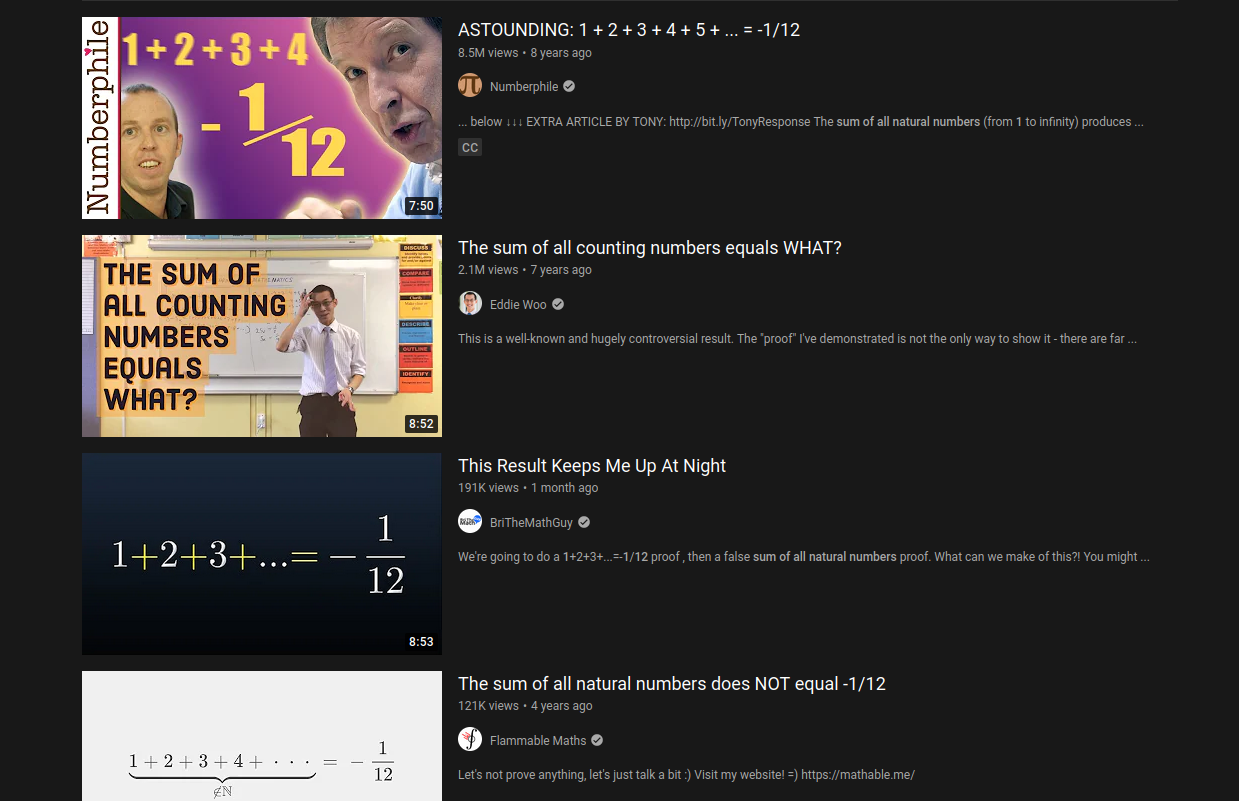
\includegraphics[width=0.7\textwidth]{youtube_screenshot.png}
        \end{center}
    \end{frame}
    \begin{frame}
        \frametitle{Riemannsche Zeta Funktion}
        \begin{equation*}
            \zeta(s)
            =
            \sum_{n=1}^{\infty}
            \frac{1}{n^s}
        \end{equation*}
        \pause
        \begin{equation*}
            \zeta(-1)
            =
            \sum_{n=1}^{\infty}
            \frac{1}{n^{-1}}
            =
            \sum_{n=1}^{\infty} n
        \end{equation*}
    \end{frame}
    \begin{frame}
        \frametitle{Originaler Definitionsbereich}
        Wir kennen die divergierende harmonische Reihe
        \begin{equation*}
            \zeta(1)
            =
            \sum_{n=1}^{\infty}
            \frac{1}{n}
            \rightarrow
            \infty,
        \end{equation*}
        und somit ist $\Re(s) > 1$.
    \end{frame}

    \section{Analytische Fortsetzung}
    \begin{frame}
        \frametitle{Plan für die Analytische Fortsetzung von $\zeta(s)$}
        \begin{center}
            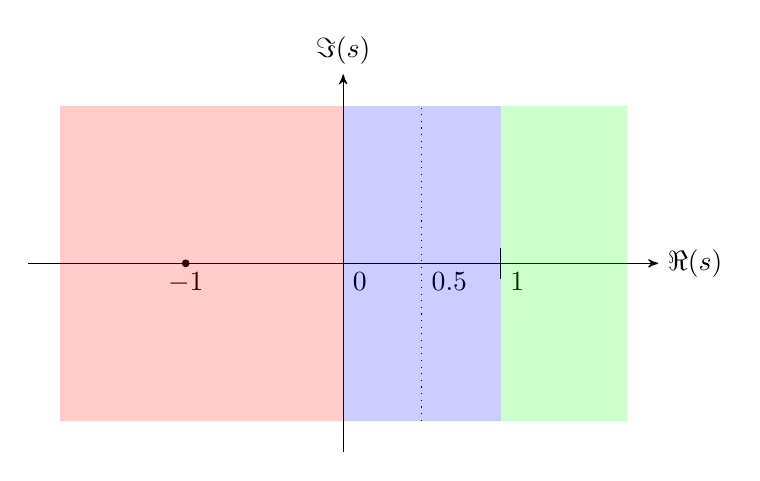
\begin{tikzpicture}[>=stealth', auto, node distance=0.9cm, scale=2,
    dot/.style={fill, circle, inner sep=0, minimum size=0.1cm}]

    \draw[->] (-2,0) -- (-1,0) node[dot]{} node[anchor=north]{$-1$} -- (0,0) node[anchor=north west]{$0$} -- (0.5,0) node[anchor=north west]{$0.5$}-- (1,0) node[anchor=north west]{$1$} -- (2,0) node[anchor=west]{$\Re(s)$};

    \draw[->] (0,-1.2) -- (0,1.2) node[anchor=south]{$\Im(s)$};
    \begin{scope}[yscale=0.1]
        \draw[] (1,-1) -- (1,1);
    \end{scope}
    \draw[dotted] (0.5,-1) -- (0.5,1);

    \begin{scope}[]
        \fill[opacity=0.2, red] (-1.8,1) rectangle (0, -1);
        \fill[opacity=0.2, blue] (0,1) rectangle (1, -1);
        \fill[opacity=0.2, green] (1,1) rectangle (1.8, -1);
    \end{scope}

\end{tikzpicture}

        \end{center}
    \end{frame}
    \begin{frame}
        \frametitle{Fortsetzung auf $\Re(s) > 0$}
        Dirichletsche Etafunktion ist
        \begin{equation*}\label{zeta:equation:eta}
            \eta(s)
            =
            \sum_{n=1}^{\infty}
            \frac{(-1)^{n-1}}{n^s},
        \end{equation*}
        und konvergiert im Bereich $\Re(s) > 0$.
    \end{frame}
    \begin{frame}
        \frametitle{Fortsetzung auf $\Re(s) > 0$}
        \begin{align}
            \zeta(s)
            &=
            \sum_{n=1}^{\infty}
            \frac{1}{n^s} \label{zeta:align1}
            \\
            \frac{1}{2^{s-1}}
            \zeta(s)
            &=
            \sum_{n=1}^{\infty}
            \frac{2}{(2n)^s} \label{zeta:align2}
        \end{align}
        \pause
        \eqref{zeta:align1} - \eqref{zeta:align2}:
        \begin{align*}
            \left(1 - \frac{1}{2^{s-1}} \right)
            \zeta(s)
            &=
            \frac{1}{1^s}
            \underbrace{-\frac{2}{2^s} + \frac{1}{2^s}}_{-\frac{1}{2^s}}
            + \frac{1}{3^s}
            \underbrace{-\frac{2}{4^s} + \frac{1}{4^s}}_{-\frac{1}{4^s}}
            \ldots
            \\
            &= \eta(s)
        \end{align*}
    \end{frame}
    \begin{frame}
        \frametitle{Fortsetzung auf $\Re(s) > 0$}
        Somit haben wir die Fortsetzung gefunden als
        \begin{equation} \label{zeta:equation:fortsetzung1}
            \zeta(s)
            :=
            \left(1 - \frac{1}{2^{s-1}} \right)^{-1} \eta(s).
        \end{equation}
    \end{frame}
    \begin{frame}
        \frametitle{Spiegelungseigenschaft für $\Re(s) < 0$}
        \begin{equation*}\label{zeta:equation:functional}
            \frac{\Gamma \left( \frac{s}{2} \right)}{\pi^{\frac{s}{2}}}
            \zeta(s)
            =
            \frac{\Gamma \left( \frac{1-s}{2} \right)}{\pi^{\frac{1-s}{2}}}
            \zeta(1-s).
        \end{equation*}
    \end{frame}
    %TODO maybe explain gamma-fct

    \section{Euler Produkt und Primzahlen}
    \begin{frame}
        \frametitle{Wieso ist die Zeta Funktion so bekannt?}
        \begin{itemize}
            \item Interessante Funktionswerte z.B. $\zeta(2) = \frac{\pi^2}{6}$
            \item Primzahlenverteilung (Riemannhypothese)
            \item Forschungsgebiet der analytischen Zahlentheorie seit dem 18. Jahrhundert
            \item ...
        \end{itemize}
    \end{frame}
    \begin{frame}
        \frametitle{Primzahlfunktion}
        \begin{center}
           \scalebox{0.5}{%% Creator: Matplotlib, PGF backend
%%
%% To include the figure in your LaTeX document, write
%%   \input{<filename>.pgf}
%%
%% Make sure the required packages are loaded in your preamble
%%   \usepackage{pgf}
%%
%% and, on pdftex
%%   \usepackage[utf8]{inputenc}\DeclareUnicodeCharacter{2212}{-}
%%
%% or, on luatex and xetex
%%   \usepackage{unicode-math}
%%
%% Figures using additional raster images can only be included by \input if
%% they are in the same directory as the main LaTeX file. For loading figures
%% from other directories you can use the `import` package
%%   \usepackage{import}
%%
%% and then include the figures with
%%   \import{<path to file>}{<filename>.pgf}
%%
%% Matplotlib used the following preamble
%%
\begingroup%
\makeatletter%
\begin{pgfpicture}%
\pgfpathrectangle{\pgfpointorigin}{\pgfqpoint{6.400000in}{4.800000in}}%
\pgfusepath{use as bounding box, clip}%
\begin{pgfscope}%
\pgfsetbuttcap%
\pgfsetmiterjoin%
\definecolor{currentfill}{rgb}{1.000000,1.000000,1.000000}%
\pgfsetfillcolor{currentfill}%
\pgfsetlinewidth{0.000000pt}%
\definecolor{currentstroke}{rgb}{1.000000,1.000000,1.000000}%
\pgfsetstrokecolor{currentstroke}%
\pgfsetdash{}{0pt}%
\pgfpathmoveto{\pgfqpoint{0.000000in}{0.000000in}}%
\pgfpathlineto{\pgfqpoint{6.400000in}{0.000000in}}%
\pgfpathlineto{\pgfqpoint{6.400000in}{4.800000in}}%
\pgfpathlineto{\pgfqpoint{0.000000in}{4.800000in}}%
\pgfpathclose%
\pgfusepath{fill}%
\end{pgfscope}%
\begin{pgfscope}%
\pgfsetbuttcap%
\pgfsetmiterjoin%
\definecolor{currentfill}{rgb}{1.000000,1.000000,1.000000}%
\pgfsetfillcolor{currentfill}%
\pgfsetlinewidth{0.000000pt}%
\definecolor{currentstroke}{rgb}{0.000000,0.000000,0.000000}%
\pgfsetstrokecolor{currentstroke}%
\pgfsetstrokeopacity{0.000000}%
\pgfsetdash{}{0pt}%
\pgfpathmoveto{\pgfqpoint{0.800000in}{0.528000in}}%
\pgfpathlineto{\pgfqpoint{5.760000in}{0.528000in}}%
\pgfpathlineto{\pgfqpoint{5.760000in}{4.224000in}}%
\pgfpathlineto{\pgfqpoint{0.800000in}{4.224000in}}%
\pgfpathclose%
\pgfusepath{fill}%
\end{pgfscope}%
\begin{pgfscope}%
\pgfsetbuttcap%
\pgfsetroundjoin%
\definecolor{currentfill}{rgb}{0.000000,0.000000,0.000000}%
\pgfsetfillcolor{currentfill}%
\pgfsetlinewidth{0.803000pt}%
\definecolor{currentstroke}{rgb}{0.000000,0.000000,0.000000}%
\pgfsetstrokecolor{currentstroke}%
\pgfsetdash{}{0pt}%
\pgfsys@defobject{currentmarker}{\pgfqpoint{0.000000in}{-0.048611in}}{\pgfqpoint{0.000000in}{0.000000in}}{%
\pgfpathmoveto{\pgfqpoint{0.000000in}{0.000000in}}%
\pgfpathlineto{\pgfqpoint{0.000000in}{-0.048611in}}%
\pgfusepath{stroke,fill}%
}%
\begin{pgfscope}%
\pgfsys@transformshift{1.025455in}{0.528000in}%
\pgfsys@useobject{currentmarker}{}%
\end{pgfscope}%
\end{pgfscope}%
\begin{pgfscope}%
\definecolor{textcolor}{rgb}{0.000000,0.000000,0.000000}%
\pgfsetstrokecolor{textcolor}%
\pgfsetfillcolor{textcolor}%
\pgftext[x=1.025455in,y=0.430778in,,top]{\color{textcolor}\sffamily\fontsize{10.000000}{12.000000}\selectfont 0}%
\end{pgfscope}%
\begin{pgfscope}%
\pgfsetbuttcap%
\pgfsetroundjoin%
\definecolor{currentfill}{rgb}{0.000000,0.000000,0.000000}%
\pgfsetfillcolor{currentfill}%
\pgfsetlinewidth{0.803000pt}%
\definecolor{currentstroke}{rgb}{0.000000,0.000000,0.000000}%
\pgfsetstrokecolor{currentstroke}%
\pgfsetdash{}{0pt}%
\pgfsys@defobject{currentmarker}{\pgfqpoint{0.000000in}{-0.048611in}}{\pgfqpoint{0.000000in}{0.000000in}}{%
\pgfpathmoveto{\pgfqpoint{0.000000in}{0.000000in}}%
\pgfpathlineto{\pgfqpoint{0.000000in}{-0.048611in}}%
\pgfusepath{stroke,fill}%
}%
\begin{pgfscope}%
\pgfsys@transformshift{1.776970in}{0.528000in}%
\pgfsys@useobject{currentmarker}{}%
\end{pgfscope}%
\end{pgfscope}%
\begin{pgfscope}%
\definecolor{textcolor}{rgb}{0.000000,0.000000,0.000000}%
\pgfsetstrokecolor{textcolor}%
\pgfsetfillcolor{textcolor}%
\pgftext[x=1.776970in,y=0.430778in,,top]{\color{textcolor}\sffamily\fontsize{10.000000}{12.000000}\selectfont 5}%
\end{pgfscope}%
\begin{pgfscope}%
\pgfsetbuttcap%
\pgfsetroundjoin%
\definecolor{currentfill}{rgb}{0.000000,0.000000,0.000000}%
\pgfsetfillcolor{currentfill}%
\pgfsetlinewidth{0.803000pt}%
\definecolor{currentstroke}{rgb}{0.000000,0.000000,0.000000}%
\pgfsetstrokecolor{currentstroke}%
\pgfsetdash{}{0pt}%
\pgfsys@defobject{currentmarker}{\pgfqpoint{0.000000in}{-0.048611in}}{\pgfqpoint{0.000000in}{0.000000in}}{%
\pgfpathmoveto{\pgfqpoint{0.000000in}{0.000000in}}%
\pgfpathlineto{\pgfqpoint{0.000000in}{-0.048611in}}%
\pgfusepath{stroke,fill}%
}%
\begin{pgfscope}%
\pgfsys@transformshift{2.528485in}{0.528000in}%
\pgfsys@useobject{currentmarker}{}%
\end{pgfscope}%
\end{pgfscope}%
\begin{pgfscope}%
\definecolor{textcolor}{rgb}{0.000000,0.000000,0.000000}%
\pgfsetstrokecolor{textcolor}%
\pgfsetfillcolor{textcolor}%
\pgftext[x=2.528485in,y=0.430778in,,top]{\color{textcolor}\sffamily\fontsize{10.000000}{12.000000}\selectfont 10}%
\end{pgfscope}%
\begin{pgfscope}%
\pgfsetbuttcap%
\pgfsetroundjoin%
\definecolor{currentfill}{rgb}{0.000000,0.000000,0.000000}%
\pgfsetfillcolor{currentfill}%
\pgfsetlinewidth{0.803000pt}%
\definecolor{currentstroke}{rgb}{0.000000,0.000000,0.000000}%
\pgfsetstrokecolor{currentstroke}%
\pgfsetdash{}{0pt}%
\pgfsys@defobject{currentmarker}{\pgfqpoint{0.000000in}{-0.048611in}}{\pgfqpoint{0.000000in}{0.000000in}}{%
\pgfpathmoveto{\pgfqpoint{0.000000in}{0.000000in}}%
\pgfpathlineto{\pgfqpoint{0.000000in}{-0.048611in}}%
\pgfusepath{stroke,fill}%
}%
\begin{pgfscope}%
\pgfsys@transformshift{3.280000in}{0.528000in}%
\pgfsys@useobject{currentmarker}{}%
\end{pgfscope}%
\end{pgfscope}%
\begin{pgfscope}%
\definecolor{textcolor}{rgb}{0.000000,0.000000,0.000000}%
\pgfsetstrokecolor{textcolor}%
\pgfsetfillcolor{textcolor}%
\pgftext[x=3.280000in,y=0.430778in,,top]{\color{textcolor}\sffamily\fontsize{10.000000}{12.000000}\selectfont 15}%
\end{pgfscope}%
\begin{pgfscope}%
\pgfsetbuttcap%
\pgfsetroundjoin%
\definecolor{currentfill}{rgb}{0.000000,0.000000,0.000000}%
\pgfsetfillcolor{currentfill}%
\pgfsetlinewidth{0.803000pt}%
\definecolor{currentstroke}{rgb}{0.000000,0.000000,0.000000}%
\pgfsetstrokecolor{currentstroke}%
\pgfsetdash{}{0pt}%
\pgfsys@defobject{currentmarker}{\pgfqpoint{0.000000in}{-0.048611in}}{\pgfqpoint{0.000000in}{0.000000in}}{%
\pgfpathmoveto{\pgfqpoint{0.000000in}{0.000000in}}%
\pgfpathlineto{\pgfqpoint{0.000000in}{-0.048611in}}%
\pgfusepath{stroke,fill}%
}%
\begin{pgfscope}%
\pgfsys@transformshift{4.031515in}{0.528000in}%
\pgfsys@useobject{currentmarker}{}%
\end{pgfscope}%
\end{pgfscope}%
\begin{pgfscope}%
\definecolor{textcolor}{rgb}{0.000000,0.000000,0.000000}%
\pgfsetstrokecolor{textcolor}%
\pgfsetfillcolor{textcolor}%
\pgftext[x=4.031515in,y=0.430778in,,top]{\color{textcolor}\sffamily\fontsize{10.000000}{12.000000}\selectfont 20}%
\end{pgfscope}%
\begin{pgfscope}%
\pgfsetbuttcap%
\pgfsetroundjoin%
\definecolor{currentfill}{rgb}{0.000000,0.000000,0.000000}%
\pgfsetfillcolor{currentfill}%
\pgfsetlinewidth{0.803000pt}%
\definecolor{currentstroke}{rgb}{0.000000,0.000000,0.000000}%
\pgfsetstrokecolor{currentstroke}%
\pgfsetdash{}{0pt}%
\pgfsys@defobject{currentmarker}{\pgfqpoint{0.000000in}{-0.048611in}}{\pgfqpoint{0.000000in}{0.000000in}}{%
\pgfpathmoveto{\pgfqpoint{0.000000in}{0.000000in}}%
\pgfpathlineto{\pgfqpoint{0.000000in}{-0.048611in}}%
\pgfusepath{stroke,fill}%
}%
\begin{pgfscope}%
\pgfsys@transformshift{4.783030in}{0.528000in}%
\pgfsys@useobject{currentmarker}{}%
\end{pgfscope}%
\end{pgfscope}%
\begin{pgfscope}%
\definecolor{textcolor}{rgb}{0.000000,0.000000,0.000000}%
\pgfsetstrokecolor{textcolor}%
\pgfsetfillcolor{textcolor}%
\pgftext[x=4.783030in,y=0.430778in,,top]{\color{textcolor}\sffamily\fontsize{10.000000}{12.000000}\selectfont 25}%
\end{pgfscope}%
\begin{pgfscope}%
\pgfsetbuttcap%
\pgfsetroundjoin%
\definecolor{currentfill}{rgb}{0.000000,0.000000,0.000000}%
\pgfsetfillcolor{currentfill}%
\pgfsetlinewidth{0.803000pt}%
\definecolor{currentstroke}{rgb}{0.000000,0.000000,0.000000}%
\pgfsetstrokecolor{currentstroke}%
\pgfsetdash{}{0pt}%
\pgfsys@defobject{currentmarker}{\pgfqpoint{0.000000in}{-0.048611in}}{\pgfqpoint{0.000000in}{0.000000in}}{%
\pgfpathmoveto{\pgfqpoint{0.000000in}{0.000000in}}%
\pgfpathlineto{\pgfqpoint{0.000000in}{-0.048611in}}%
\pgfusepath{stroke,fill}%
}%
\begin{pgfscope}%
\pgfsys@transformshift{5.534545in}{0.528000in}%
\pgfsys@useobject{currentmarker}{}%
\end{pgfscope}%
\end{pgfscope}%
\begin{pgfscope}%
\definecolor{textcolor}{rgb}{0.000000,0.000000,0.000000}%
\pgfsetstrokecolor{textcolor}%
\pgfsetfillcolor{textcolor}%
\pgftext[x=5.534545in,y=0.430778in,,top]{\color{textcolor}\sffamily\fontsize{10.000000}{12.000000}\selectfont 30}%
\end{pgfscope}%
\begin{pgfscope}%
\pgfsetbuttcap%
\pgfsetroundjoin%
\definecolor{currentfill}{rgb}{0.000000,0.000000,0.000000}%
\pgfsetfillcolor{currentfill}%
\pgfsetlinewidth{0.803000pt}%
\definecolor{currentstroke}{rgb}{0.000000,0.000000,0.000000}%
\pgfsetstrokecolor{currentstroke}%
\pgfsetdash{}{0pt}%
\pgfsys@defobject{currentmarker}{\pgfqpoint{-0.048611in}{0.000000in}}{\pgfqpoint{-0.000000in}{0.000000in}}{%
\pgfpathmoveto{\pgfqpoint{-0.000000in}{0.000000in}}%
\pgfpathlineto{\pgfqpoint{-0.048611in}{0.000000in}}%
\pgfusepath{stroke,fill}%
}%
\begin{pgfscope}%
\pgfsys@transformshift{0.800000in}{0.696000in}%
\pgfsys@useobject{currentmarker}{}%
\end{pgfscope}%
\end{pgfscope}%
\begin{pgfscope}%
\definecolor{textcolor}{rgb}{0.000000,0.000000,0.000000}%
\pgfsetstrokecolor{textcolor}%
\pgfsetfillcolor{textcolor}%
\pgftext[x=0.633333in, y=0.647775in, left, base]{\color{textcolor}\sffamily\fontsize{10.000000}{12.000000}\selectfont 0}%
\end{pgfscope}%
\begin{pgfscope}%
\pgfsetbuttcap%
\pgfsetroundjoin%
\definecolor{currentfill}{rgb}{0.000000,0.000000,0.000000}%
\pgfsetfillcolor{currentfill}%
\pgfsetlinewidth{0.803000pt}%
\definecolor{currentstroke}{rgb}{0.000000,0.000000,0.000000}%
\pgfsetstrokecolor{currentstroke}%
\pgfsetdash{}{0pt}%
\pgfsys@defobject{currentmarker}{\pgfqpoint{-0.048611in}{0.000000in}}{\pgfqpoint{-0.000000in}{0.000000in}}{%
\pgfpathmoveto{\pgfqpoint{-0.000000in}{0.000000in}}%
\pgfpathlineto{\pgfqpoint{-0.048611in}{0.000000in}}%
\pgfusepath{stroke,fill}%
}%
\begin{pgfscope}%
\pgfsys@transformshift{0.800000in}{1.368000in}%
\pgfsys@useobject{currentmarker}{}%
\end{pgfscope}%
\end{pgfscope}%
\begin{pgfscope}%
\definecolor{textcolor}{rgb}{0.000000,0.000000,0.000000}%
\pgfsetstrokecolor{textcolor}%
\pgfsetfillcolor{textcolor}%
\pgftext[x=0.633333in, y=1.319775in, left, base]{\color{textcolor}\sffamily\fontsize{10.000000}{12.000000}\selectfont 2}%
\end{pgfscope}%
\begin{pgfscope}%
\pgfsetbuttcap%
\pgfsetroundjoin%
\definecolor{currentfill}{rgb}{0.000000,0.000000,0.000000}%
\pgfsetfillcolor{currentfill}%
\pgfsetlinewidth{0.803000pt}%
\definecolor{currentstroke}{rgb}{0.000000,0.000000,0.000000}%
\pgfsetstrokecolor{currentstroke}%
\pgfsetdash{}{0pt}%
\pgfsys@defobject{currentmarker}{\pgfqpoint{-0.048611in}{0.000000in}}{\pgfqpoint{-0.000000in}{0.000000in}}{%
\pgfpathmoveto{\pgfqpoint{-0.000000in}{0.000000in}}%
\pgfpathlineto{\pgfqpoint{-0.048611in}{0.000000in}}%
\pgfusepath{stroke,fill}%
}%
\begin{pgfscope}%
\pgfsys@transformshift{0.800000in}{2.040000in}%
\pgfsys@useobject{currentmarker}{}%
\end{pgfscope}%
\end{pgfscope}%
\begin{pgfscope}%
\definecolor{textcolor}{rgb}{0.000000,0.000000,0.000000}%
\pgfsetstrokecolor{textcolor}%
\pgfsetfillcolor{textcolor}%
\pgftext[x=0.633333in, y=1.991775in, left, base]{\color{textcolor}\sffamily\fontsize{10.000000}{12.000000}\selectfont 4}%
\end{pgfscope}%
\begin{pgfscope}%
\pgfsetbuttcap%
\pgfsetroundjoin%
\definecolor{currentfill}{rgb}{0.000000,0.000000,0.000000}%
\pgfsetfillcolor{currentfill}%
\pgfsetlinewidth{0.803000pt}%
\definecolor{currentstroke}{rgb}{0.000000,0.000000,0.000000}%
\pgfsetstrokecolor{currentstroke}%
\pgfsetdash{}{0pt}%
\pgfsys@defobject{currentmarker}{\pgfqpoint{-0.048611in}{0.000000in}}{\pgfqpoint{-0.000000in}{0.000000in}}{%
\pgfpathmoveto{\pgfqpoint{-0.000000in}{0.000000in}}%
\pgfpathlineto{\pgfqpoint{-0.048611in}{0.000000in}}%
\pgfusepath{stroke,fill}%
}%
\begin{pgfscope}%
\pgfsys@transformshift{0.800000in}{2.712000in}%
\pgfsys@useobject{currentmarker}{}%
\end{pgfscope}%
\end{pgfscope}%
\begin{pgfscope}%
\definecolor{textcolor}{rgb}{0.000000,0.000000,0.000000}%
\pgfsetstrokecolor{textcolor}%
\pgfsetfillcolor{textcolor}%
\pgftext[x=0.633333in, y=2.663775in, left, base]{\color{textcolor}\sffamily\fontsize{10.000000}{12.000000}\selectfont 6}%
\end{pgfscope}%
\begin{pgfscope}%
\pgfsetbuttcap%
\pgfsetroundjoin%
\definecolor{currentfill}{rgb}{0.000000,0.000000,0.000000}%
\pgfsetfillcolor{currentfill}%
\pgfsetlinewidth{0.803000pt}%
\definecolor{currentstroke}{rgb}{0.000000,0.000000,0.000000}%
\pgfsetstrokecolor{currentstroke}%
\pgfsetdash{}{0pt}%
\pgfsys@defobject{currentmarker}{\pgfqpoint{-0.048611in}{0.000000in}}{\pgfqpoint{-0.000000in}{0.000000in}}{%
\pgfpathmoveto{\pgfqpoint{-0.000000in}{0.000000in}}%
\pgfpathlineto{\pgfqpoint{-0.048611in}{0.000000in}}%
\pgfusepath{stroke,fill}%
}%
\begin{pgfscope}%
\pgfsys@transformshift{0.800000in}{3.384000in}%
\pgfsys@useobject{currentmarker}{}%
\end{pgfscope}%
\end{pgfscope}%
\begin{pgfscope}%
\definecolor{textcolor}{rgb}{0.000000,0.000000,0.000000}%
\pgfsetstrokecolor{textcolor}%
\pgfsetfillcolor{textcolor}%
\pgftext[x=0.633333in, y=3.335775in, left, base]{\color{textcolor}\sffamily\fontsize{10.000000}{12.000000}\selectfont 8}%
\end{pgfscope}%
\begin{pgfscope}%
\pgfsetbuttcap%
\pgfsetroundjoin%
\definecolor{currentfill}{rgb}{0.000000,0.000000,0.000000}%
\pgfsetfillcolor{currentfill}%
\pgfsetlinewidth{0.803000pt}%
\definecolor{currentstroke}{rgb}{0.000000,0.000000,0.000000}%
\pgfsetstrokecolor{currentstroke}%
\pgfsetdash{}{0pt}%
\pgfsys@defobject{currentmarker}{\pgfqpoint{-0.048611in}{0.000000in}}{\pgfqpoint{-0.000000in}{0.000000in}}{%
\pgfpathmoveto{\pgfqpoint{-0.000000in}{0.000000in}}%
\pgfpathlineto{\pgfqpoint{-0.048611in}{0.000000in}}%
\pgfusepath{stroke,fill}%
}%
\begin{pgfscope}%
\pgfsys@transformshift{0.800000in}{4.056000in}%
\pgfsys@useobject{currentmarker}{}%
\end{pgfscope}%
\end{pgfscope}%
\begin{pgfscope}%
\definecolor{textcolor}{rgb}{0.000000,0.000000,0.000000}%
\pgfsetstrokecolor{textcolor}%
\pgfsetfillcolor{textcolor}%
\pgftext[x=0.563888in, y=4.007775in, left, base]{\color{textcolor}\sffamily\fontsize{10.000000}{12.000000}\selectfont 10}%
\end{pgfscope}%
\begin{pgfscope}%
\pgfpathrectangle{\pgfqpoint{0.800000in}{0.528000in}}{\pgfqpoint{4.960000in}{3.696000in}}%
\pgfusepath{clip}%
\pgfsetrectcap%
\pgfsetroundjoin%
\pgfsetlinewidth{1.505625pt}%
\definecolor{currentstroke}{rgb}{0.121569,0.466667,0.705882}%
\pgfsetstrokecolor{currentstroke}%
\pgfsetdash{}{0pt}%
\pgfpathmoveto{\pgfqpoint{1.025455in}{0.696000in}}%
\pgfpathlineto{\pgfqpoint{1.175758in}{0.696000in}}%
\pgfpathlineto{\pgfqpoint{1.175758in}{0.696000in}}%
\pgfpathlineto{\pgfqpoint{1.326061in}{0.696000in}}%
\pgfpathlineto{\pgfqpoint{1.326061in}{1.032000in}}%
\pgfpathlineto{\pgfqpoint{1.476364in}{1.032000in}}%
\pgfpathlineto{\pgfqpoint{1.476364in}{1.368000in}}%
\pgfpathlineto{\pgfqpoint{1.626667in}{1.368000in}}%
\pgfpathlineto{\pgfqpoint{1.626667in}{1.368000in}}%
\pgfpathlineto{\pgfqpoint{1.776970in}{1.368000in}}%
\pgfpathlineto{\pgfqpoint{1.776970in}{1.704000in}}%
\pgfpathlineto{\pgfqpoint{1.927273in}{1.704000in}}%
\pgfpathlineto{\pgfqpoint{1.927273in}{1.704000in}}%
\pgfpathlineto{\pgfqpoint{2.077576in}{1.704000in}}%
\pgfpathlineto{\pgfqpoint{2.077576in}{2.040000in}}%
\pgfpathlineto{\pgfqpoint{2.227879in}{2.040000in}}%
\pgfpathlineto{\pgfqpoint{2.227879in}{2.040000in}}%
\pgfpathlineto{\pgfqpoint{2.378182in}{2.040000in}}%
\pgfpathlineto{\pgfqpoint{2.378182in}{2.040000in}}%
\pgfpathlineto{\pgfqpoint{2.528485in}{2.040000in}}%
\pgfpathlineto{\pgfqpoint{2.528485in}{2.040000in}}%
\pgfpathlineto{\pgfqpoint{2.678788in}{2.040000in}}%
\pgfpathlineto{\pgfqpoint{2.678788in}{2.376000in}}%
\pgfpathlineto{\pgfqpoint{2.829091in}{2.376000in}}%
\pgfpathlineto{\pgfqpoint{2.829091in}{2.376000in}}%
\pgfpathlineto{\pgfqpoint{2.979394in}{2.376000in}}%
\pgfpathlineto{\pgfqpoint{2.979394in}{2.712000in}}%
\pgfpathlineto{\pgfqpoint{3.129697in}{2.712000in}}%
\pgfpathlineto{\pgfqpoint{3.129697in}{2.712000in}}%
\pgfpathlineto{\pgfqpoint{3.280000in}{2.712000in}}%
\pgfpathlineto{\pgfqpoint{3.280000in}{2.712000in}}%
\pgfpathlineto{\pgfqpoint{3.430303in}{2.712000in}}%
\pgfpathlineto{\pgfqpoint{3.430303in}{2.712000in}}%
\pgfpathlineto{\pgfqpoint{3.580606in}{2.712000in}}%
\pgfpathlineto{\pgfqpoint{3.580606in}{3.048000in}}%
\pgfpathlineto{\pgfqpoint{3.730909in}{3.048000in}}%
\pgfpathlineto{\pgfqpoint{3.730909in}{3.048000in}}%
\pgfpathlineto{\pgfqpoint{3.881212in}{3.048000in}}%
\pgfpathlineto{\pgfqpoint{3.881212in}{3.384000in}}%
\pgfpathlineto{\pgfqpoint{4.031515in}{3.384000in}}%
\pgfpathlineto{\pgfqpoint{4.031515in}{3.384000in}}%
\pgfpathlineto{\pgfqpoint{4.181818in}{3.384000in}}%
\pgfpathlineto{\pgfqpoint{4.181818in}{3.384000in}}%
\pgfpathlineto{\pgfqpoint{4.332121in}{3.384000in}}%
\pgfpathlineto{\pgfqpoint{4.332121in}{3.384000in}}%
\pgfpathlineto{\pgfqpoint{4.482424in}{3.384000in}}%
\pgfpathlineto{\pgfqpoint{4.482424in}{3.720000in}}%
\pgfpathlineto{\pgfqpoint{4.632727in}{3.720000in}}%
\pgfpathlineto{\pgfqpoint{4.632727in}{3.720000in}}%
\pgfpathlineto{\pgfqpoint{4.783030in}{3.720000in}}%
\pgfpathlineto{\pgfqpoint{4.783030in}{3.720000in}}%
\pgfpathlineto{\pgfqpoint{4.933333in}{3.720000in}}%
\pgfpathlineto{\pgfqpoint{4.933333in}{3.720000in}}%
\pgfpathlineto{\pgfqpoint{5.083636in}{3.720000in}}%
\pgfpathlineto{\pgfqpoint{5.083636in}{3.720000in}}%
\pgfpathlineto{\pgfqpoint{5.233939in}{3.720000in}}%
\pgfpathlineto{\pgfqpoint{5.233939in}{3.720000in}}%
\pgfpathlineto{\pgfqpoint{5.384242in}{3.720000in}}%
\pgfpathlineto{\pgfqpoint{5.384242in}{4.056000in}}%
\pgfpathlineto{\pgfqpoint{5.534545in}{4.056000in}}%
\pgfusepath{stroke}%
\end{pgfscope}%
\begin{pgfscope}%
\pgfsetrectcap%
\pgfsetmiterjoin%
\pgfsetlinewidth{0.803000pt}%
\definecolor{currentstroke}{rgb}{0.000000,0.000000,0.000000}%
\pgfsetstrokecolor{currentstroke}%
\pgfsetdash{}{0pt}%
\pgfpathmoveto{\pgfqpoint{0.800000in}{0.528000in}}%
\pgfpathlineto{\pgfqpoint{0.800000in}{4.224000in}}%
\pgfusepath{stroke}%
\end{pgfscope}%
\begin{pgfscope}%
\pgfsetrectcap%
\pgfsetmiterjoin%
\pgfsetlinewidth{0.803000pt}%
\definecolor{currentstroke}{rgb}{0.000000,0.000000,0.000000}%
\pgfsetstrokecolor{currentstroke}%
\pgfsetdash{}{0pt}%
\pgfpathmoveto{\pgfqpoint{5.760000in}{0.528000in}}%
\pgfpathlineto{\pgfqpoint{5.760000in}{4.224000in}}%
\pgfusepath{stroke}%
\end{pgfscope}%
\begin{pgfscope}%
\pgfsetrectcap%
\pgfsetmiterjoin%
\pgfsetlinewidth{0.803000pt}%
\definecolor{currentstroke}{rgb}{0.000000,0.000000,0.000000}%
\pgfsetstrokecolor{currentstroke}%
\pgfsetdash{}{0pt}%
\pgfpathmoveto{\pgfqpoint{0.800000in}{0.528000in}}%
\pgfpathlineto{\pgfqpoint{5.760000in}{0.528000in}}%
\pgfusepath{stroke}%
\end{pgfscope}%
\begin{pgfscope}%
\pgfsetrectcap%
\pgfsetmiterjoin%
\pgfsetlinewidth{0.803000pt}%
\definecolor{currentstroke}{rgb}{0.000000,0.000000,0.000000}%
\pgfsetstrokecolor{currentstroke}%
\pgfsetdash{}{0pt}%
\pgfpathmoveto{\pgfqpoint{0.800000in}{4.224000in}}%
\pgfpathlineto{\pgfqpoint{5.760000in}{4.224000in}}%
\pgfusepath{stroke}%
\end{pgfscope}%
\end{pgfpicture}%
\makeatother%
\endgroup%
}
        \end{center}
    \end{frame}
    \begin{frame}
        \frametitle{Zusammenhang Zeta und Primzahlen}
        %TODO
    \end{frame}


    \section{Weitere Eigenschaften}



\end{document}

